\setAuthor{Mihkel Kree}
\setRound{lõppvoor}
\setYear{2012}
\setNumber{G 2}
\setDifficulty{4}
\setTopic{Dünaamika}

\prob{Veejuga}
Pildil on foto horisontaalsest torust väljuva veejoaga ning teljestik, mille
väikseim jaotis on võrdne veejoa läbimõõduga selle algkõrgusel. Ühtlase
kiirusega voolava veejoa alla pandud mõõteklaas ruumalaga
$V=\SI{150}{cm^3}$ täitus ajaga $t=\SI{5}{min}$. Leidke
toru siseläbimõõt.
\begin{center}
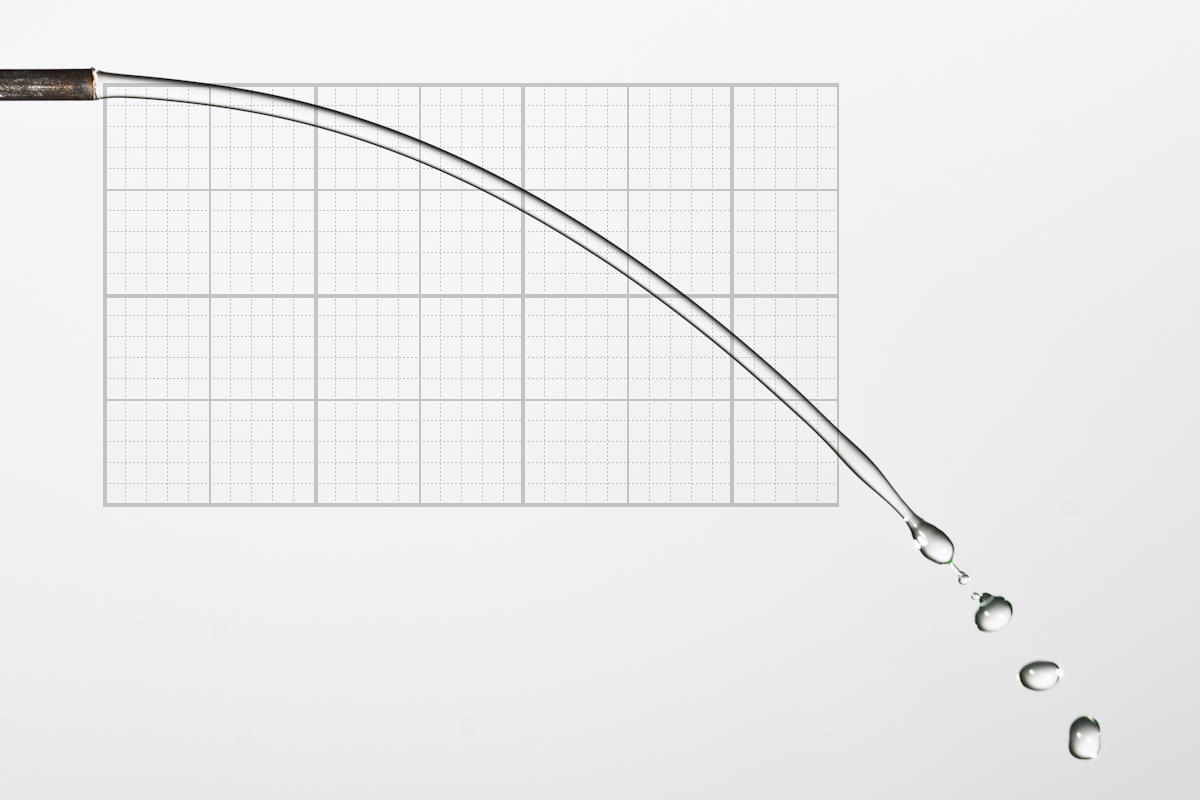
\includegraphics[width=0.7\linewidth]{2012-v3g-02-jet}%
\end{center}

\hint
Torust väljuv vesi liigub nagu vabalt langev keha horisontaalsuunalise algkiirusega $v$. Seega on veejuga parabooli kujuga, mille parameetrid saab jooniselt mõõta.

\solu
Vaatleme torust väljuvat veeosakest kui vabalt langevat keha horisontaalsuunalise algkiirusega $v$, mille horisontaalsuunaline kaugus kasvab ajas lineaarselt $s=vt$, vertikaalsuunaline aga kui $h=\frac{1}{2}gt^2$. Järelikult $h\sim s^2$ ning veejoa kuju on matemaatiliselt kirjeldatav parabooli võrrandiga $y=kx^2$, kus $x$ ja $y$ on veejoa koordinaadid joonisel toodud teljestiku ühikutes (nullpunktiks valime teljestiku ülemise vasakpoolse nurga, $x$-telg olgu suunatud paremale ning $y$-telg alla). Määramaks joonise abil võrdetegurit $k$, valime mõned täisarvuliste koordinaatiga punktid $(x,y)$, millest juga läbi läheb, näiteks $(\num{19,5})$, $(\num{24,8})$ ja $(\num{34,16})$. Arvutades iga punkti jaoks suhte $x^2/y$, leiame et $k=\num{0.014}$. 
	
Arvestades järgnevalt, et teljestiku ühikule vastab füüsikaline pikkus $d$ (veejoa läbimõõt, mille loeme võrdseks toru sisediameetriga), võime teisendada kaugused $s$ ja $h$ teljestiku ühikutesse:
\[x=\frac{s}{d}=\frac{vt}{d},\quad \mathrm{ja} \quad y=\frac{h}{d}=\frac{gt^2}{2d}=\frac{gd}{2v^2}\frac{v^2t^2}{d^2}=\frac{gd}{2v^2}x^2,\]
millest saame kiirust ja diameetrit omavahel siduva võrrandi
\begin{equation}\label{eq:2012-v3g-02-vd1}
k=\frac{gd}{2v^2}\quad \mathrm{ehk} \quad \frac{v^2}{d}=\frac{g}{2k}.
\end{equation}
	
Nüüd arvestame aja $t$ jooksul torust läbi voolanud vee ruumalaks $Svt$, kus $S$ on toru sisepindala, millest saame teise kiirust ja diameetrit sisaldava võrrandi
\begin{equation}\label{eq:2012-v3g-02-vd2}
V=\frac{\pi d^2}{4}vt \quad \mathrm{ehk} \quad vd^2=\frac{4V}{\pi t}.
\end{equation}

Võttes võrrandi (\ref{eq:2012-v3g-02-vd2}) ruutu ning jagades läbi võrrandiga (\ref{eq:2012-v3g-02-vd1}), taandub kiirus välja ning alles jääb
\[d^5=\frac{16V^2}{\pi^2t^2}\frac{2k}{g}, \quad \mathrm{millest} \quad d=\left(\frac{32V^2k}{\pi^2 t^2 g}\right)^{\frac{1}{5}}=\SI{1}{mm	}.\]

\probeng{Water spurt}
In the figure below there is a photo of a water spurt flowing out of a horizontal tube and a coordinate grid, the grid’s smallest unit is equal to the water spurt’s diameter on its initial height. A measuring cup of volume $V=\SI{150}{cm^3}$ is placed below the spurt, which is flowing with even speed.  It takes $t=\SI{5}{min}$ for the cup to fill completely. Find the tube’s inner diameter.
\begin{center}
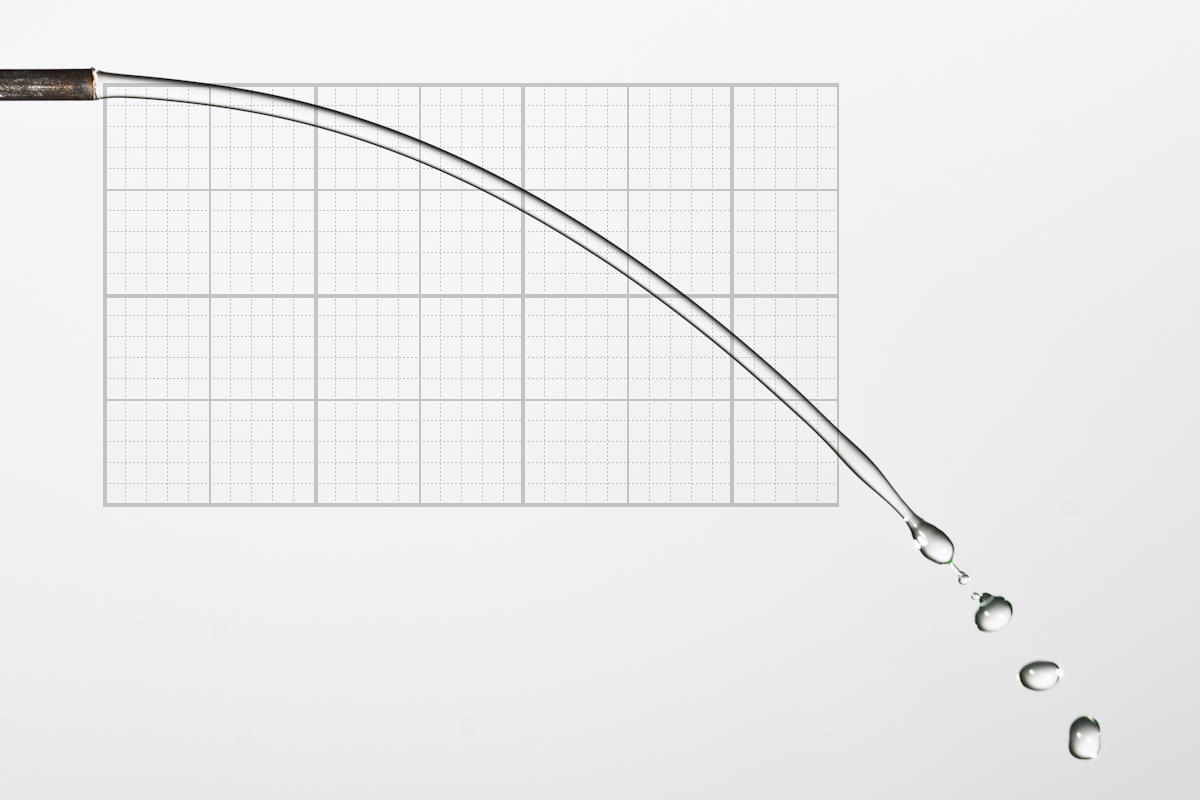
\includegraphics[width=0.7\linewidth]{2012-v3g-02-jet}%
\end{center}

\hinteng
The water exiting the tube moves like a free falling body with a horizontally directed initial speed $v$. Thus, the water spurt is shaped like a parabola, the parameters of it can be measured in the figure.

\solueng
Let us observe a part of water exiting the tube as a freely falling body with initial velocity $v$ directed along the horizontal. The horizontal distance of the part increases linearly in time $s=vt$, but the vertical as $h=\frac{1}{2}gt^2$. Thus, $h\sim s^2$ and the shape of the water spurt is mathematically described by the parabola’s equation $y=kx^2$ where $x$ and $y$ are the coordinates of the water spurt in the units of the figure’s coordinate system (we choose the origin to be the upper left corner, let the $x$-axis be directed to the right and the $y$-axis to down). To determine the constant of proportionality $k$ with the help of the figure we choose some points $(x,y)$ with integer coordinates that the spurt goes through, for example $(\num{19,5})$, $(\num{24,8})$ and $(\num{34,16})$. Calculating the ratio $x^2/y$ for each point we find that $k=\num{0.014}$.\\
Considering next that a unit of the frame of reference is equal to the physical length $d$ (the diameter of the spurt that we assume to be equal to the inner diameter of the tube), we can transform the distances $s$ and $h$ into the units of the frame of reference:
\[x=\frac{s}{d}=\frac{vt}{d},\quad \mathrm{and} \quad y=\frac{h}{d}=\frac{gt^2}{2d}=\frac{gd}{2v^2}\frac{v^2t^2}{d^2}=\frac{gd}{2v^2}x^2,\] 
where we can get an equation that includes both the velocity and diameter
\begin{equation}\label{eq:2012-v3g-02-vd1}
k=\frac{gd}{2v^2}\quad \mathrm{meaning} \quad \frac{v^2}{d}=\frac{g}{2k}.
\end{equation} 
The volume of water going through the tube during the time $t$ is $Svt$ where $S$ is the inner area of the tube. From this we get a second equation that includes the velocity and diameter
\begin{equation}\label{eq:2012-v3g-02-vd2}
V=\frac{\pi d^2}{4}vt \quad \mathrm{meaning} \quad vd^2=\frac{4V}{\pi t}.
\end{equation} 
Squaring the equation (2) and dividing it by the equation (1) the velocity cancels out and we get
\[d^5=\frac{16V^2}{\pi^2t^2}\frac{2k}{g}, \quad \mathrm{from which} \quad d=\left(\frac{32V^2k}{\pi^2 t^2 g}\right)^{\frac{1}{5}}=\SI{1}{mm	}.\]
\probend